\documentclass[11pt]{article}

\def\articlename{固定收益}
\def\authorname{杨弘毅}
\def\startdate{2021年9月5日}

\ifx \authorname\undefined
  \def\authorname{杨弘毅}
\else
\fi

\author{\authorname}
\date{创建:\startdate \\修改:\today}

\usepackage[a4paper,left=6em,right=6em]{geometry}
\usepackage{amsmath,amsfonts,amsthm,bbold}
\usepackage{booktabs,float,multirow}
\usepackage{cancel}
\usepackage{enumitem}
\usepackage{multicol}
\usepackage{graphicx}
\usepackage[toc,title]{appendix}
\usepackage{tikz}
\usetikzlibrary{arrows.meta}
\usetikzlibrary{patterns}
\usetikzlibrary{decorations.pathreplacing}
\usetikzlibrary{decorations.pathmorphing}
\usepackage{subcaption}
\usepackage{fancyhdr}
\pagestyle{fancy}
\setlength{\headheight}{15pt}
\usepackage{footmisc}
\usepackage{hyperref}
\usepackage{tocloft}
\hypersetup{
    colorlinks=true, %set true if you want colored links
    linkcolor=blue,
    linktoc=all, %set to all if you want both sections and subsections linked
    citecolor=black,
    filecolor=black,
    urlcolor=blue
}
\usepackage[UTF8]{ctex}

\title{\articlename}

% Format
\setlength{\cftbeforesecskip}{6pt}
\setlength{\parskip}{0.6em}
\renewcommand{\baselinestretch}{1.4}
\setlist{noitemsep,itemindent=1em,topsep=0em,leftmargin=4em,rightmargin=4em}
\setlist[2]{leftmargin=2em}

% Shortcut
\newcommand{\divider}{\vspace{-\parskip}\noindent\rule{\linewidth}{0.4pt}}
\newcommand{\tops}[1]{\texorpdfstring{#1}{TEXT}}

% Theorem
\newtheorem{thm}{定理}[section] 
\newtheorem{proposition}[thm]{命题}
\newtheorem{lemma}[thm]{引理}
\newtheorem{corollary}[thm]{推论}
\newtheorem{property}[thm]{性质}
\newtheorem{example}[thm]{例子}
\newtheorem{remark}[thm]{备注}
\newtheorem{note}[thm]{注释}

% Symbol
\newcommand{\E}{\mathbb{E}}
\newcommand{\mcl}{\mathcal{L}}
\newcommand{\rnE}{\widetilde{\mathbb{E}}}
\newcommand{\wt}[1]{\widetilde{#1}}
\DeclareMathOperator{\Var}{Var}
\DeclareMathOperator{\Cov}{Cov}
\newcommand{\abs}[1]{\left\lvert #1\right\rvert}
\newcommand{\norm}[1]{\left\lVert #1\right\rVert}
\newcommand{\given}{\:\vert\:}

\begin{document}
\maketitle
\tableofcontents
% \newpage

\section{基本概念}

\subsection{复利}

单利(Simple interest)与复利(Compound interest)的差别在于之前产生的利息是否进入下一期的计算(即不考虑利息的时间价值),若进入下一期的计算则为复利。
\begin{example}
    假设一个存入1000元,名义年利率为4\%,每年4次付息,那么有在四年后,单利可获得:
    \begin{equation*}
        1000 + 1000 \times \frac{4\%}{4} \times 4 \times 4 = 1160 
    \end{equation*}

    复利可获得:
    \begin{equation*}
        1000 \times ( 1 + \frac{4\%}{4})^{4 \times 4} = 1172.57
    \end{equation*}
\end{example}

对于在一年内多次付息,若一年支付$12\%$,那么半年付息将分两次支付,每次支付$6\%$。假设面值为1000,那么在半年的时候将获得$1000 \times \frac{0.12}{2} = 60$利息,与之前本金相加得到$1060$。此时到年末,假设本金与利息都将获得$6\%$的利息,那么就有$1060 \times \frac{0.12}{2} = 63.60$,即最终将获得$1000 \times (1+\frac{0.12}{2})^2 = 1123.60$。因此在这个例子里,名义利率(Nominal rate)为$10\%$,而实际年利率或有效年利率(Effective annual rate,EAR或Annual equivalent rate,AER)则为$\frac{1123.60}{1000}-1 = 12.36\%$,可见计息频率增加,导致实际年化利率上升。

\begin{example}
    当名义利率为$12\%$时,有实际年利率为:
    \begin{table}[H]
    \centering
    \begin{tabular}{@{}lll@{}}
    \toprule
    频率(m) & 实际利率 & 实际年化利率 \\ \midrule
    1(一年)   & $\frac{0.12}{1}=0.12$  & $(1.12)^1-1=0.12$ \\
    2(半年)   & $\frac{0.12}{2}=0.06$  & $(1.06)^2-1=0.1236$      \\
    4(季度)   & $\frac{0.12}{4}=0.03$  & $(1.03)^4-1=0.125509$       \\
    12(月度)  & $\frac{0.12}{12}=0.01$ & $(1.01)^{12}-1=0.126162$ \\
    52(周度)  & $\frac{0.12}{52}=0.0023$  & $(1.0023)^{52}-1=0.127341$\\
    365(日度) & $\frac{0.12}{365}=0.00033$ & $(1.00033)^{365}-1=0.127475$ \\
    $\infty$ (连续)  & \multicolumn{2}{l}{$ \lim_{m \rightarrow \infty} (1+\frac{0.12}{m})^{m} - 1 = e^{0.12} - 1 = 0.127497
    $}            \\ \bottomrule
    \end{tabular}
    \end{table}
\end{example}

假设平价发行的债券,票面利率为12,面值为12,当计息频率为1时,即按年计息,则有:
\begin{equation*}
    1000 = \frac{1120}{(1+0.12)^1}
\end{equation*}

当计息频率为2时,使用名义利率进行贴现:
\begin{equation*}
    1000 = \frac{60}{(1+\frac{0.12}{2})^1} + \frac{1060}{(1+\frac{0.12}{2})^2}
\end{equation*}

或使用实际年化利率进行贴现:
\begin{equation*}
    1000 = \frac{60}{(1+0.1236)^{0.5}} + \frac{1060}{(1+0.1236)^1}
\end{equation*}

可以看到计算实际年化利率的过程即为将利率变化为以年为频率的过程。

\subsection{久期}

久期(Duration)衡量利率变动(1\%)对债券价格的影响,即衡量债券对利率的敏感程度(Sensitivity)或暴露(Exposure),即衡量了利率风险的大小(Interest rate risk)。那么高久期意味着利率变动对债券价格影响大,或债券价格对利率变动更敏感。反之,对于第久期的债券,利率变动对其影响较小。
\begin{itemize}
    \item 期限影响:债券期限越长,受到利率影响更大,则久期越大。相反,债券期限越短,受到利率影响更小,久期越小。假设一笔隔夜偿还的债券,和一笔十年偿还的债券,显然期限更长的债券受利率影响更大。
    \item 票息影响:票息越小,那么更少的金额在最终到期之前被支付,因而久期越大。假设一个零息债券,只有一笔本金在到期日支付,此时所有的现金流都在到期日,那么受利率影响最大。相反,票息越大,现金流越在期限内平摊开来,久期越小。
\end{itemize}

\subsection*{麦考利久期}

一般情况下提到久期一般指麦考利久期(Macaulay Duration),对于一个支付n期票息债券,$CF_i$为每一期现金流,y为到期收益率(YTM),M为面值额债券,此时每一期的现值$PV_i$应有$\text{PV}_i = \frac{\text{CF}_i}{(1+y)^i}$。此时债券现值TPV(Total Present Value)为所有现金流现值之和,用P表示:
\begin{equation*}
    P = \sum_{i=1}^{n} \text{PV}_i = \sum_{i=1}^{n} \frac{\text{CF}_i}{(1+y)^i}
\end{equation*}

此时定义麦考利久期如下:
\begin{align*}
    \text{MacD} &= \frac{\sum_{i=1}^{n} t_i \times PV_i}{P}
    = \sum_{i=1}^{n} \left( t_i \times \frac{PV_i}{P} \right) \\
    &= \left[ \frac{1 \text{CF}_1}{(1+y)^1} + \frac{2\text{CF}_2}{(1+y)^2} + \dots + \frac{n \text{CF}_n}{(1+y)^{n}} \right] \frac{1}{P}
\end{align*}

可以看到事实上久期计算的为加权平均的债券期限,其中权重为每一笔现金流现值占所有现金流现值的比值。若使用连续复利计算(Continuously compounded),则有:
\begin{gather*}
    P = \sum_{i=1}^{n} \text{PV}_i = \sum_{i=1}^{n} \text{CF}_i e^{-y t_i} \\
    \text{MacD} = \sum_{i=1}^{n} t_i \frac{\text{CF}_i e^{-y t_i}}{P}
\end{gather*}

\begin{example}
    假设如下图所示两年期面值为100的债券,半年一次支付票息,票面利率为20\%,到期收益率为3.9605\%。此时该债券的麦考瑞久期应有:
    \begin{align*}
        \text{MacD} &= \left[ 0.5 \times \frac{10}{(1+0.039605)^{0.5}}
        + 1 \times \frac{10}{(1+0.039605)^{1}} \right. \\
        & \qquad \left. + 1.5 \times \frac{10}{(1+0.039605)^{1.5}}
        + 2 \times \frac{110}{(1+0.039605)^{2}} \right] \frac{1}{P} \\
        &= \frac{0.5 \times 9.81 + 1 \times 9.62 + 1.5 \times 9.43 + 2 \times 101.78}{9.81 + 9.62 + 9.43 + 101.78} \\
        &\approx 1.78
    \end{align*}
\end{example}

\begin{figure}[H]
    \centering
    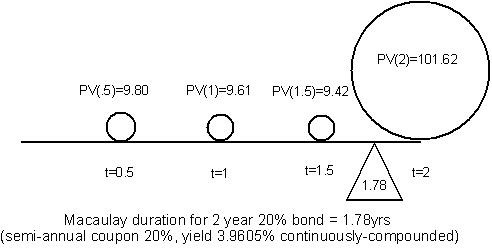
\includegraphics[width=0.6\textwidth]{fig/duration.jpeg}
    \caption{久期}
    \label{fig:duration}
\end{figure}

麦考利久期的计算方式与计算重心(Center of mass)的方式相同,实质为计算所有现金流现值($PV_i$)的重心位置。重心的计算公式(一维)有如下所示($m$为每个部分的重量,$x$为距离):
\begin{equation*}
    x_{cm} = \frac{m_1 x_1 + m_2 x_2 + \dots + m_n x_n}{m_1 + m_2 + \dots + m_n}
\end{equation*}

\subsection*{修正久期}

麦考利久期只是衡量了利率风险的相对大小,即一个10年久期的债券,比5年久期的债券风险更大,而修正久期就对其进行了量化。例如:当修正久期为3时,利率每上涨1\%,将使得债券价格下跌3\%。因此定义修正久期(Modified duration)为对于利率变化债券价格变化的百分比:
\begin{equation*}
    \text{ModD} = -\frac{1}{P} \frac{\partial P}{\partial y} = \frac{\partial \ln P}{\partial y}
\end{equation*}

当复利计算频率为1,由上可知:
\begin{equation*}
    P = \sum_{i=1}^{n} \text{PV}_i = \sum_{i=1}^{n} \frac{\text{CF}_i}{(1+y)^i}
    = \frac{\text{CF}_1}{(1+y)^1} + \frac{\text{CF}_2}{(1+y)^2} + \dots + \frac{\text{CF}_n}{(1+y)^{n}}
\end{equation*}

对y求导可得:
\begin{equation*}
    \frac{\partial P}{\partial y} = \frac{(-1)\text{CF}_1}{(1+y)^2} + \frac{(-2)\text{CF}_2}{(1+y)^3} + \dots + \frac{(-n)\text{CF}_n}{(1+y)^{n+1}}
\end{equation*}

将$\frac{-1}{(1+y)}$提出,等式两边同乘$\frac{1}{P}$,可以看到后半部分为麦考利久期:
\begin{align*}
    \frac{\partial P}{\partial y} \frac{1}{P} &= -\frac{1}{1+y} \left[ \frac{\text{CF}_1}{(1+y)^1} + \frac{2\text{CF}_2}{(1+y)^2} + \dots + \frac{n \text{CF}_n}{(1+y)^{n}} \right] \frac{1}{P} \\
    &= -\frac{1}{1+y} \times \text{MacD}
\end{align*}

同时,由于$\text{ModD} = -\frac{1}{P} \frac{\partial P}{\partial y}$,因此可以得到:
\begin{equation*}
    \text{ModD} = \frac{\text{MacD}}{1+y}
\end{equation*}

当$y_k$为名义利率时,假设$k$为复利计算频率(1为每年,2为每半年...),$t_i$为票息支付时间(年,如2年半年付息债券则有$t_i=0.5,1.0,1.5,2.0$):
\begin{equation*}
    P = \sum_{i=1}^{n} \text{PV}_i = \sum_{i=1}^{n} \frac{\text{CF}_i}{(1+y_k/k)^{k t_i}}
\end{equation*}

由定义可知,其麦考利久期为:
\begin{equation*}
    \text{MacD} = \sum_{i=1}^{n} \frac{t_i}{P} \frac{\text{CF}_i}{(1+y_k/k)^{k t_i}}
\end{equation*}

如同对修正久期的推导可得,
\begin{equation*}
    \frac{\partial P}{\partial y_k} = - \frac{1}{1+y_k/k} \sum_{i=1}^{n} t_i \frac{\text{CF}_i}{(1+y_k/k)^{k t_i}} = - \frac{\text{MacD} \times P}{1 + y_k/k}
\end{equation*}

因此:
\begin{equation*}
    \text{ModD} = \frac{\text{MacD}}{1+y_k/k}
\end{equation*}

可以看到当使用连续复利进行计算时,即$k=\infty$时,有麦考利久期与修正久期相等$\text{ModD} = \text{MacD}$。同时也可以通过连续复利进行贴现证明,当使用连续复利计算时,由上可知:
\begin{equation*}
    P = \text{CF}_1 e^{-y1} + \text{CF}_2 e^{-y2} + \dots + \text{CF}_n e^{-yn}
\end{equation*}

同样对y求导,
\begin{equation*}
    \frac{dP}{dy} = -1 \text{CF}_1 e^{-y1} -2 \text{CF}_2 e^{-y2} - \dots -n \text{CF}_n e^{-yn}
\end{equation*}

并同乘$-\frac{1}{P}$,同时根据久期的定义,同样可以发现当使用连续复利进行计算时,麦考利久期与修正久期相等。
\begin{align*}
    \text{ModD} = - \frac{dP}{dy} \frac{1}{P} = \frac{1}{P} \left[ 1 \text{CF}_1 e^{-y1} +2 \text{CF}_2 e^{-y2} + \dots -n \text{CF}_n e^{-yn} \right]
    = \text{MacD}
\end{align*}

由于可以使用$\frac{P(y+\Delta y) - P(y-\Delta y)}{2\Delta y}$估计$\frac{\partial P}{\partial y}$,因此也可以用如下公式估算修正久期:
\begin{equation*}
    \text{ModD} \approx - \frac{P(y+\Delta y) - P(y-\Delta y)}{2 P \Delta y}
\end{equation*}

因此对于y较小的变化,可近似认为(即假定债券价格随着利率线性变化):
\begin{equation*}
    \frac{\Delta P}{P} \approx - \text{ModD} \times \Delta y
\end{equation*}

\begin{example}
    假设一个期限为8年的债券,每年付息,票息为5\%,其到期收益率为6\%。

    \begin{table}[H]
    \centering
    \begin{tabular}{@{}crrrr@{}}
    \toprule
    \textbf{期数} & \multicolumn{1}{c}{\textbf{现金流}} & \multicolumn{1}{c}{\textbf{现值}} & \multicolumn{1}{c}{\textbf{权重}} & \multicolumn{1}{c}{\textbf{期数乘权重}} \\ \midrule
    1 & 50 & 47.17 & 5.03\% & 0.05 \\
    2 & 50 & 44.50 & 4.74\% & 0.09 \\
    3 & 50 & 41.98 & 4.48\% & 0.13 \\
    4 & 50 & 39.60 & 4.22\% & 0.17 \\
    5 & 50 & 37.36 & 3.98\% & 0.20 \\
    6 & 50 & 35.25 & 3.36\% & 0.23 \\
    7 & 50 & 33.25 & 3.55\% & 0.25 \\
    8 & 1050 & 658.78 & 70.24\% & 5.62 \\ \midrule
    \textbf{合计} & \textbf{} & \textbf{937.90} & \textbf{100\%} & \textbf{6.74} \\ \bottomrule
    \end{tabular}
    \end{table}

    此时可以看到麦考利久期$\text{MacD} = 6.74$,并有修正久期$\text{ModD} = \frac{\text{MacD}}{1+y} = \frac{6.74}{1.06} = 6.36$。那么此时对于利率变动$\pm 1\%$,应有债券价格变动约$\mp 6.36\%$,即$937.90 \times 6.36\% = 59.65$(假设为线性变化)。
\end{example}


\subsection{凸性调整}

凸性(Convexity),可以看到事实上的债券价格与利率变化并非线性关系,因此若只使用久期判断将产生误差。

\begin{figure}[H]
    \centering
    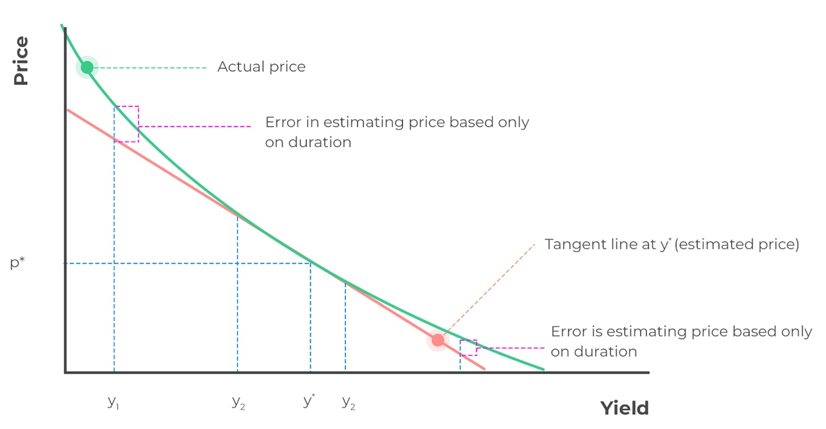
\includegraphics[width=0.8\textwidth]{fig/duration-convexity.png}
    \caption{久期与凸性}
    \label{fig:duration-convexity}
\end{figure}

\begin{equation*}
    \%\Delta\text{PV} = -\text{ModD} \times \Delta\text{Yield} + \frac{1}{2} \times \text{Convexity} \times (\Delta\text{Yield})^2
\end{equation*}

其中:
\begin{equation*}
    \text{Covexity} \approx \frac{V_{+}+V_{-}-2 V_0}{(\Delta\text{Yield}^2 V_0)}
\end{equation*}


\subsection{即期利率、远期利率、到期收益率}

即期利率(Spot rate):从t时刻开始,到T时刻到期,所有现金流只发生在T时刻的投资回报率。因而也常常被称为零息利率(zero-coupon interest rate or zero rate)或称零息收益率(zero-coupon yield)。同时即期利率与贴现因子是一一对应的,贴现因子只是即期利率的另一种表达。

到期收益率(Yield-tomaturity,YTM):$y_t^T$为从t时刻开始,到T时刻到期,投资的年化平均内含回报率(或内部收益率Internal rate of return,即使得NPV为0的收益率),可以看做是即期利率的一种加权平均,与债券价格一一对应。若相比两个期限、Coupon不同的债券,对比其YTM可以衡量其真实债券收益的多少。另外由于一般最后一笔现金流权重较大,因此到期收益率与即期收益率较为接近。具体而言,每一年都以一个相同的利率贴现,而即期利率每个时间段不同。假设一个2年到期,每年末付息的债券,那么有使用即期利率进行贴现,与使用YTM进行贴现结果应相同:
\begin{equation*}
    \frac{C_1}{1+s_{0,1}} +\frac{C_2+P}{1+s_{0,2}} = 
    \frac{C_1}{1+y_{0,2}} +\frac{C_3+P}{(1+y_{0,2})^2}
\end{equation*}

对于使用连续复利,使用到期收益率计算,可以看到每期使用利率$y_t^{t_n}$不变:
\begin{equation*}
    V_{t_0}^{t_n} = C_1 e^{-y_{t_0,t_n}(t_1-t_0)} + C_2 e^{-y_{t_0,t_n}(t_2-t_0)}
    + \dots + C_n e^{-y_{t_0,t_n}(t_n-t_0)}
    = \sum_{i=1}^{n} C_i e^{-y_{t_0,t_n}\times (t_i-t_0)}
\end{equation*}

使用即期利率进行计算,对于不同时间跨度的贴现利率不同:
\begin{equation*}
    V_{t_0}^{t_n} = C_1 e^{-s_{t_0,t_1}(t_1-t_0)} + C_2 e^{-s_{t_0,t_2}(t_2-t_0)}
    + \dots + C_n e^{-s_{t_0,t_n}(t_n-t_0)}
    = \sum_{i=1}^{n} C_i e^{-s_{t_0,t_i}\times (t_i-t_0)}
\end{equation*}

远期利率(Forward rate)可视为边际利率,即对于上行的期限结构,远期利率高于长期利率。相反,对于下降的利率期限结构,那么远期利率低于长期利率。假设三个时间节点$t_0,t_1,t_2$,连续复利有可得:
\begin{equation*}
    e^{r_{t_0,t_1}(t_1-t_0)} \times e^{r_{t_1,t_2}(t_2-t_1)} = e^{r_{t_0,t_2}(t_2-t_0)}
\end{equation*}

那么此时远期利率$r_{t_1,t_2}$有:
\begin{gather*}
    r_{t_0,t_1}(t_1-t_0) + r_{t_1,t_2}(t_2-t_1) = r_{t_0,t_2}(t_2-t_0) \\
    r_{t_1,t_2}(t_2-t_1) = r_{t_0,t_2}(t_2-t_0) - r_{t_0,t_1}(t_1-t_0) \\
    r_{t_1,t_2} = \frac{r_{t_0,t_2}(t_2-t_0) - r_{t_0,t_1}(t_1-t_0)}{(t_2-t_1)}
\end{gather*}

期货利率:本质与远期利率相同,通过期货合约规定未来一定期限的利率,但在交易机制设计上,使得两者有一定的差异。远期利率协议报价为利率,而利率期货报价一般为价格,期货利率隐含在报价中(100-利率=94,那么利率为6\%),因此两者多头也不同,远期利率,多头规避利率上升风险。而期货利率多头(价格上涨),规避利率下跌风险。

债券报价时使用净价而非全价:
\begin{itemize}
    \item 全价(full price):现金价格(cash price)或发票价格(invoice price)
    \item 净价(clean price):等于全价减去应计利息(accrued interest),避免报价不连续(由于票息)
\end{itemize}

\subsection{Riding Yield Curve}

期限结构骑乘,由于期限结构是向上倾斜的,当假设持有期期限结构不变时,自然roll down或riding yiled curve,即。即利率下行,债券价格上涨。

当想投资两年期的固定收益债券时,假设投资2年的债券,并持有到期。也可以投资一个期限更长的债券,并持有两年,获得更高的收益。


\section{利率模型导论}

\subsection{利率期限结构模型分类}

利率的期限结构(term structure of interest rates),又通俗的称为收益率曲线(yield curve),收益率和期限关系的曲线。
\begin{itemize}
    \item 动态模型
    \begin{itemize}
        \item 均衡模型(Equilibrium Model):输入为经济变量,输出为利率水平,例如:Vasicek,CIR模型
        \item 无套利模型(No arbitrage Model):输入为利率水平,输出为相关金融工具的价格,例如:Hull\&White,HJM模型
    \end{itemize}
    \item 静态模型
    \begin{itemize}
        \item Nelson-Siegel模型
    \end{itemize}
\end{itemize}

\subsection{动态模型与静态模型的对比}

静态模型建模目的在于拟合当前时点市场利率期限结构,追求高拟合度、曲线的平滑以及拟合的灵活度和稳定度,关注其统计以及数学上的性质。无法推断未来的参数变化与今天的参数是如何关联的,因此成为“静态”模型。动态模型目的在于刻画期限结构未来分布(利率期限结构以及利率波动率),并可为衍生品定价。 

\subsection{关于利率期限模型}

债券的定价只需要使用DCF即可以求得,并不需要复杂的利率模型。提出利率模型(又如零息债债券定价模型)的目的是使用当前可观测到即期利率(或债券价格),求模型内的(隐含)参数,倒推瞬时利率(利用瞬时利率可得到整条利率期限结构),为没有交易的产品进行定价。如使用BSM模型可以估计波动率。

\subsection{关于因子}

因子可以是纯数学因子,或有经济含义的因子。如宏观金融(Macro-Finance)模型的因子:宏观经济增长、通货膨胀、货币政策、剩下的归结到数学因子。非张成(unspanned),仅有部分宏观信息(Y)被模型之中因子(X)所解释(即反应在利率曲线中)。而没有进入因子的部分,或未反应在利率曲线中的部分,对于未来债券收益率有预测力。

\subsection{关于风险价格}

在利率模型中,风险价格($\lambda$)的重要性来源于利率的不可交易性。对于可交易的资产,由现实测度转换至风险中性测度下,人们对风险并无偏好,所以风险溢酬为零,根据无套利条件,其漂移率等于预期收益率等于无风险利率。而利率作为不可交易资产,想使用风险中性测度,其漂移率为$\mu_t-\lambda\sigma_t$,风险量可认为是个客观变量,但风险价格,或单位风险的所要求风险溢酬却是主观的。
为了研究无限维的即期利率或其中包含的远期利率,采用了对瞬时即期利率和瞬时远期利率的建模的方法进行降维,需要对瞬时利率或瞬时远期进行研究,由于其不可观测,无法在现实测度下研究。只能通过定价公式,建立起现实可观测的债券价格,与不可观测的瞬时利率或瞬时远期利率之间的关系,从可观测的债券价格中提取信息,刻画利率期限结构,则需要牵涉不同的测度。使用风险中性测度,是为了更好研究利率的特性,也可以使用其他测度,是数学的变换,而风险中性测度有具体的经济含义,如风险价格、风险厌恶等。对于仿射模型,也需要认为设置风险价格,使其在现实测度以及风险中性测度下均保持仿射模型良好的数学性质。

\section{动态模型(Dynamic Term Structure Models,DTSMs)}

动态模型可以用于帮助了解利率期限结构中的静态和动态特征,了解未来利率变化的分布(时间序列以及横截面)。对于复杂的含权类固定收益产品而言,近拟合当前利率期限结构的静态模型已经不足以为其定价。相对于不含权的简单利率产品,利率衍生品的价格不仅取决于当前利率的期限结构,还取决于利率的波动率。对于诸如债券、利率远期、利率期货和利率互换等进行定价,可以仅依靠静态模型进行定价。而对于利率期权产品,还需要考虑利率波动的信息,而由于期权产品并非线性,因此需要动态模型进行建模。使用不同的期限结构模型对不同的产品进行定价,存在模型风险,而使用统一的模型(动态模型)进行不仅可对利率期权定价,也可对线性的其他利率产品进行定价。由此可以在公司企业内部建立起统一、一致的定价框架,以确保利率风险管理体系的一致性。

使用随机过程为股票价格建模,在时间点t,股票价格$S_t$仅有一个取值。而在对于利率模型,在任意时间点,如研究的对象为Shibor,可为ON、1W、2W、1M等至1Y期限的即期利率等等,即在利率期限结构上有无限的维度,可视为$R_t$为不同期限即期利率组成的向量,还需要研究其在时间序列上的变化。并且由于利率的不可直接交易的特性(交易的是债券以及利率的衍生品等),使得无法借用风险中性测度对利率进行建模,因为只有可交易的资产在风险中性测度下的漂移率为预期收益率,即无风险利率。而对于非可交易资产,风险中性下的漂移率为$\mu_t-\lambda\sigma_t$(现实测度下漂移率-风险价格(每单位风险的风险溢酬)*风险数量,或现实测度下漂移率-风险溢酬)。由于利率不可交易漂移率并非预期收益率,加之风险溢酬难以测量,因此使用风险中性测度对利率进行建模难以使用。(零息债可以使用风险中性测度,因为可交易)

使用动态模型进行建模对象可为无限维即期利率(远期利率),对应着无限维的零息债。或为一维瞬时即期利率(instantaneous spot rate或short rate),也可为无限维瞬时远期利率。一维瞬时即期利率可视为整条利率曲线(期限结构)的基本元素,只要其变化规律已知,就可以张成不同期限(无限维)的即期利率(不同到期期限的零息债券价格)。或可理解为将整条无限维度的向量(不同期限的利率),降维成一个变量(瞬时利率$r_t$,单因子或多因子模型为有限维)。瞬时远期利率为无限维,如ON之后的瞬时远期利率或1M之后的瞬时远期。对于零息债券的贴现,可以使用未来的瞬时即期利率不断进行贴现(为随机变量,需要在风险中心测度下求其期望)。而使用瞬时即期利率,则隐含在当前的即期利率之中,为当前已知,不需要使用风险中性测度期望。因此需要在一维的瞬时即期利率(需使用风险中性测度)和无限维的瞬时远期利率(不需要使用风险中性测度)之中进行取舍。需要注意的是一般不使用债券价值作为建模对象,因为债券到期回到其面值,使用随机过程显然不合适,需要使用到布朗桥。

\subsection{实用注意标准}

模型需要反映现实市场中观察到的利率动态特征:
\begin{itemize}
    \item 利率的均值回归特征
    \item 利率的基本分布特征:肥尾和非对称分布
    \item 利率期限结构长短端变动不一致,如利率上升短端上升幅度较大,长端上升幅度较小,利率期限结构趋于水平 。反之,当利率下降,利率期限结构变得更加陡峭
    \item 利率波动率特征:与利率水平有关,当利率较高时,波动率较大
\end{itemize}

\subsection{动态利率模型分类}

\begin{itemize}
    \item \textbf{单因子模型与多因子模型}:单一或者多个风险源($dW_t$),单因子利率期限结构的静态形状不够丰富;主成分分析表明,几乎所有市场的无风险利率曲线都至少收到2-3个不相关重要因素的影响
    \item \textbf{时间齐次和时间非齐次}:均衡模型为时间齐次,波动率不为时间的函数(波动率因时间而发生改变经济含义较弱)。一般无套利模型为时间非齐次,波动率为时间的函数。(单因子时间齐次仿射模型中,时间齐次与当前时间点无关,而与剩余期限有关 )
    \item \textbf{连续模型与带跳模型}:是否存在跳跃
    \item \textbf{扩散模型与非扩散模型}:扩散过程,即飘移项($\mu(X(t),t)$)与方差项($\sigma(X(t),t)$)都为$X_t$(自身)的函数函数
    \item \textbf{仿射模型与非仿射模型}:$\mu(X(t),t)$为$X(t)$和$t$的仿射函数(线性函数$\mu=a+bX_t$),$\sigma(X(t),t)$的方差(而非标准差)为仿射函数(或波动项的平方为线性,几何布朗运动非线性,波动项的平方为$\sigma^2$),仿射模型优点为数学上容易求解(得到解析解),而缺点则为无法捕捉非线性。
\end{itemize}

\subsection{均衡模型(Equilibrium model)(绝对定价)}

均衡模型注重于经济逻辑,对所有市场参与者的偏好和禀赋进行显性假设,通过债券的供需均衡确定债券价格和利率水平(CIR模型为均衡模型的代表,通过供需均衡推导出随机过程)。后期模型未必进行推导,但用一些基于偏好的基本假设,这些模型的假设是和市场均衡兼容,即认为是均衡模型。经典的均衡模型多为时间齐次模型,有有限参数的模型刻画无限维时变的利率期限结构(利率曲线)。均衡模型与债券的价格拟合度低,不适用于定价,多用于刻画市场利率的一般变化规律。

单因子、时间齐次、连续过程、扩散过程、仿射模型
\begin{align*}
	dr_t &= \mu_t(r_t)dt+\sigma_t(r_t)dZ_t \\
	dr_t &= \kappa(\theta-r_t)dt+\sqrt{\omega_0+\omega_1 r_t}dZ_t
\end{align*}

\subsubsection{Merton(1973)模型}

\noindent
\begin{equation*}
	dr_t = \tilde{\mu_t}(r_t)dt+\sigma_t(r_t)d\tilde{Z_t}
\end{equation*}

可认为是上述模型的特例,参数均为常数。开创性的将随机过程引入利率领域,对Merton模型的拓展产生了后续众多的动态利率模型。提出了风险中性测度下瞬时利率服从普通布朗运动(正态分布,可能出现负利率,次贷危机之后才有负利率,才可能是正态分布)

\subsubsection{Vasicek(1977)模型}

瞬时利率在现实测度下服从均值回复(O-U过程,Ornstein-Uhlenbeck process)模型
\begin{equation*}
	dr_t = \kappa(\theta-r_t)dt+\sigma dZ_t
\end{equation*}

风险中性下需要对风险价格(单位风险溢酬)设定,使得在风险中性测度下保持Vasicek模型:
\begin{align*}
	dr_t &= [\kappa(\theta-r_t)-\lambda_t\sigma]dt+\sigma dZ_t \\
	&= \tilde{\kappa}(\tilde{\theta}-r_t)dt+\sigma d\tilde{Z_t}
\end{align*}

静态特征:长其均值收敛,参数取值不同,可以得到不同的利率期限结构形态

动态特征:剩余期限的不同,即期利率对瞬时利率的敏感程度(瞬时利率的系数)不同,剩余期限短变化幅度大($\tfrac{\beta(t,T)}{T-t}$),短期利率波动率大于长期利率波动率

\subsubsection{Cox-Ingersoll-Ross(1985)模型}

瞬时利率在现实服从均值回复平方根模型,通过对投资与融资的一般均衡的分析得到,而非人为设定:
\begin{equation*}
	dr_t = \kappa(\theta-r_t)dt+\sigma\sqrt{r_t} dZ_t
\end{equation*}

$dZ_t$为正态分布,乘上瞬时利率的平方根为卡方分布,加上其他参数的约束条件,能保证瞬时利率大于零(解决了Vasicek模型负利率的问题)。如果风险价格设定满足特定形式(如$\lambda_t=b\sqrt{r_t}$),可使得瞬时利率在风险中性测度下仍回服从CIR过程:
\begin{equation*}
	dr_t = \tilde{\kappa}(\tilde{\theta}-r_t)dt+\sigma\sqrt{r_t} d\tilde{Z_t}
\end{equation*}

静态特征与动态特征:保留Vasicek模型的优点

改进Vasicek模型,避免负利率;改进了Vasicek中波动率与利率水平无关的缺陷,利率越高,利率波动率越高;

\subsubsection{其他模型}

\begin{itemize}
    \item Beagleholde and Tenney(1991)(两因子Vasicek模型)
    \item Hull and White(1994)(两因子Vasicek模型)
    \item Longstaff-Schwartz(1992)
\end{itemize}

\subsubsection{时间序列估计法(极大似然估计、矩估计)}

使用历史利率数据进行估计,没有使用债券价格,而使用利率本身。因此没有使用定价模型,建立债券价格和瞬时利率之间的关系。得到的是现实测度的参数,而非风险中性下的参数和风险价格。只能用于刻画现实市场(观测到的)中利率的动态特征,因为没使用定价模型,不能用于定价,也无法得到利率风险溢酬相关信息。使用1个月或3个月的国债机器利率作为瞬时利率的代理变量,存在误差。只研究特定到期期限的利即期利率,得到时间序列上的特征,而无法刻画整条利率期限结构曲线的动态特征(横截面信息)。

\subsubsection{横截面估计法(校准法)}

在给定时刻,选取横截面上的高流动性债券或其他固定收益证券数据,使得模型得到的价值贴近市场价格,求得一组参数值,即定价误差的平方和最小。对于选取得每一个时刻,横截面均有一组最优参数,并没有捕捉其时间序列上的特征,完全忽略了时间序列维度上的动态特征。由于每天进行校准都有一组参数,因此未时间非齐次,随着时间变化。此时得到得是定价测度下得参数,多为风险中性测度参数($\kappa$,$\theta$,$\phi$),无法得到显示测度下得漂移率和风险价格,只能用于为其他利率产品定价,无法刻画现实市场中的利率特征。

\subsubsection{面板估计}

方法一:用时间序列估计现实测度参数,再以这些参数作为输入,根据横截面市场价格确定风险中性参数($\mu$与$\tilde{\mu}$两者之差得到了风险溢酬,可用于确定风险价格)

方法二:与方法一前后顺序相反,先使用横截面数据得到风险中性参数,再以这些参数作为输入,使用时间序列数据得到现实参数和风险价格。

方法三:卡尔曼滤波(Kalman filter)方法和MCMC(Markov chain Monte Carlo)方法同时估计时间序列与横截面信息,得到的参数既可用于定价,也可用于刻画利率动态特征。但对于一段时间内的样本只能得到最优化的一组参数,并不能适应动态变化的市场需要,因此通常也只用于刻画现实市场中利率的动态特征,较少用于定价。
简单而言,卡尔曼滤波由两部分方程组成:第一部分为观测方程,为包含自变量与因变量关系的方程,用于检测两者横截面上的特征;第二部分为状态方程,描述自变量(状态变量,不可观测)在时间序列上的变化。卡尔曼滤波的算法是由预测与更新两部分交替互相迭代进行。在预测步骤中,卡尔曼滤波会通过状态方程(自变量时间序列上的变化)产生有关目前状态的估计。只要观察到下一时刻的因变量的变化(其中一定含有某种程度的误差,包括随机噪声)。通过度量观测因变量(真实值)与预测估计值之间的残差,利用加权平均的方法更新估计值。给与确定性越高的测量加权比重也越高,反之确定性越低权重月底。即将预测估计值分布(正态分布)和观测值分布(正态分布)进行加权平均,得到新的下一时刻的新的预测值分布(正态分布),从此完成迭代,最终能得到一组最优的参数,使得估计的结果最优。这样就得到了状态方程中,关于自变量变化的现实测度下的参数,以及观测方程中,自变量(因子)与因变量(债券价格)风险中性定价模型中的风险中性测度下参数,由此同时估计现实测度与风险中性测度下的所有参数。得到最优参数之后,还能通过卡尔曼平滑的方法,得到最优的自变量(不可观测)取值。

\subsection{无套利模型(No-arbitrage model)(相对定价)}

无套利模型注重于贴近市场,不追求解释利率曲线均衡水平是如何形成的,直接以市场数据作为模型输入,基于无套利条件建立模型,使模型与市场数据吻合,可用已知产品的市场价格为没有在市场上交易的产品定价。

\subsubsection{校准的均衡模型}

由于均衡模型有较好的经济含义,但难以用于定价。通过校准,使得模型估计值与市场的观察值相接近,使得均衡模型可用于定价。使得均衡模型中的参数(飘移项或波动项参数)变为时间非齐次(时变函数,随时间变化而变化),保证模型能够较好的拟合每天的市场信息。如果不希望模型过度拉扯,不希望校准波动率数据,而只校准利率数据,则波动率有关的所有参数都应该室时间齐次的。缺点为使用已有的均衡模型进行拟合,可能使得参数中存在较强的时变性质,而减少了原模型的经济内涵。多因子模型也可进行校准,但多因子模型自身已经由多个参数,使其能较好的适应各种情形,使得对多因子模型校准的意义不大。

\subsubsection{Ho-Lee(1986)}

在Dybvig(1988)中证明其连续形式为:
\begin{align*}
	dr_t &= \tilde{\mu}(t) + \sigma d\tilde{Z_t} \\
	\tilde{\mu}(t) &= \frac{\partial f^t_0}{\partial t} + \sigma^2 t
\end{align*}

与Merton模型相比,波动率为常数,但漂移率为时变($f_0$为远期利率),变为时间非齐次,通过远期利率曲线进行校准。使用时变的飘移率为无套利接口,在每个时刻使用市场利率曲线作为模型的输入数据,使得该模型与市场无风险利率曲线仍然是天然拟合的。模型较为简单,但缺点为并未改进Merton模型的缺陷。

\subsubsection{Hull-White(1990,1994a)}

单因子模型由Vasick模型演变而来,使用长期均值$\tilde{\phi}(t)$为无套利接口,模型简单,但缺点也并未改善Vasicek模型的缺陷:
\begin{align*}
	dr_t &= \tilde{\kappa}(\tilde{\varphi}(t)-r_t)dt+\sigma d\tilde{Z_t} \\
	\tilde{\varphi}(t) &= f^t_0 + \frac{1}{\tilde{\kappa}}\frac{\partial f^t_0}{\partial t} + \frac{\sigma^2}{2\tilde{\kappa}^2} (1-e^{-2\tilde{\kappa}t})
\end{align*}

双因子模型由双因子Vasicek模型演变而来,其中长期均值由两部分组成:$\tilde{\phi}(t)$为无套利接口,$\phi(t)$为随机过程。长期利率与短期利率由各自的风险源(两者相关),但未改变原模型正态分布的假设。
\begin{align*}
	dr_t &= \left(\tilde{\varphi}(t) + \varphi_t - \tilde{\kappa}r_t \right) dt + \sigma d\tilde{Z}_{1,t} \\
	d\varphi_t &= -\tilde{\kappa_\varphi}\varphi_t dt + \sigma_\varphi \rho d\tilde{Z}_{1,t} + \sigma_{\varphi}\sqrt{1-\rho^2} d\tilde{Z}_{2,t}\\
	\tilde{\varphi}(t) &= \frac{\partial f^t_0}{\partial t} + \tilde{\kappa}_r f^t_0 + \frac{\partial \xi(0,t)}{\partial t} + \tilde{\kappa}_r \xi(0,t)
\end{align*}

\subsubsection{BDT(1990)}

Black,Derman and Toy(1990),除了仿射模型之外,非仿射模型也可通过动态校准参数转化为无套利模型,而模型复杂度进一步提升,使得对零息债都没有解析解,只能通过数值方法求解。在BDT模型中,不仅漂移率为时变,波动率也是时变的,使用二叉树(使用利率对数波动率),同时拟合每个时刻市场的利率期限结构与波动率期限结构。使用一年期的零息债到期收益率(或即期利率)作为瞬时利率的代理变量。在保证中间的节点重合的情况下,n时刻(开始时刻为0时刻),有$n+1$个待估节点,减少节点数量。要求在同一时刻中间节点($i-1$个)波动率应该相等,可写出$i-1$个方程。并通过拟合$i+1$年期灵犀债券收益率和波动率,可再写出2个方程。

Hull and White(1990)指出BDT模型的连续形式,实际为假设瞬时利率对数服从三个参数都室时间非齐次的Vasicek模型:
\begin{align*}
	d\ln r_t & = \left[ \tilde{\varphi}(t) + \frac{1}{\sigma(t)} \frac{\partial \sigma(t)}{\partial t} \ln r_t \right] + \sigma(t) d\tilde{Z}_t \\
	&= \frac{1}{\sigma(t)} \frac{\partial \sigma(t)}{\partial t} \left[ \tilde{\varphi}(t)\left( \frac{1}{\sigma(t)} \frac{\partial \sigma(t)}{\partial t} \right)^{-1} + \ln r_t \right]dt + \sigma(t)d\tilde{Z}_t
\end{align*}
$\tilde{\varphi}(t)$为无套利接口,长期均值由$\tilde{\varphi}(t)$与$\sigma(t)$决定,可以发现$\sigma(t)$同时决定了瞬时利率对数的波动率与均值回复速度($\tilde{\kappa}$)。即模型中只有两个待估参数$\tilde{\varphi}(t)$与$\sigma(t)$,这两个时变的参数由t时刻市场数据校准得到。

与Hull-White单因子模型相比,BDT模型不仅可以拟合当前市场利率期限结构,还可以拟合当前利率波动率的期限结构。并使用瞬时利率的对数进行建模,避免了负利率的可能,且实现过程相对简单。由于均值回复速度完全由波动率觉得,不一定合理。为了追求拟合利率期限结构与波动率期限结构,所有参数都为时间非齐次,可能存在为了拟合数据而过度拉扯模型。且假设波动率为时间非齐次,即认为波动率因时间变化而变化并不合理,可能因为其他因素变化,而非时间流逝。

\subsubsection{BK(1991)}

Black and Karasinski(1991),对BDT模型一般化:
\begin{equation*}
	d\ln r_t = \tilde{\kappa}\left(\tilde{\mu}(t) - \ln r_t \right) dt + \sigma(t)d\tilde{Z}_t
\end{equation*}
使用了独立的均值回复速度$\tilde{\kappa}$,灵活性提高,样本内拟合效果提高,但使用的市场信息也相应增加,且样本外的定价和预测结构并不必然优于BDT模型。

\subsubsection{HJM(1992)}

HJM模型为典型的无套利相对定价模型框架。在构建动态利率模型时就引入无套利要求,初始要求为使得模型产生的初始利率曲线就与当前市场利率期限结构相一致,因此构建出来的模型自然就是无套利的相对定价模型。由于一开始已经使用了利率期限结构信息,因此该模型不能再为普通债券定价,只能用于其他利率衍生品的定价。如前所述,债券定价只需要使用DCF模型即可,使用动态利率模型时为了求得模型内部参数,再为其他利率产品定价。

HJM模型使用瞬时远期利率作为建模对象,瞬时远期利率与瞬时利率都为利率期限结构的最基本元素:
\begin{equation*}
	B^T_t = e^{-\int^T_t f^u_t du} \quad\Rightarrow\quad 
	\ln B^T_t = - \int^T_t f^u_t du \quad\Rightarrow\quad
	R^T_t = - \frac{-\int^T_t f^u_t du}{T-t}
\end{equation*}

\begin{equation*}
	f^T_t = -\frac{\partial \ln B^T_t}{\partial T} = R^T_t + (T-t)\frac{\partial y^T_t}{\partial T}
\end{equation*}

由于使用了瞬时远期,因此并不需要涉及风险中性下的期望,且瞬时远期利率与瞬时利率的关系最为简单:
\begin{equation*}
	r_t = f^t_t = \lim_{T\rightarrow t} R^T_t = -\lim_{T\rightarrow t} \frac{\partial B^t_t}{\partial T}
\end{equation*}

经过推导,得到风险中性测度下的瞬时远期利率的漂移率为:
\begin{equation*}
	\tilde{\mu}^T_{f,t} = \sum^n_{i=1} \sigma^T_{fi,t} \int^T_t \sigma^u_{fi,t} du
\end{equation*}

只跟波动率有关,不需要估计漂移率,规避了需要估计漂移率的问题(涉及风险溢酬、风险价格等信息)。因此说明在使用瞬时远期利率时,可以使用风险中性测度为利率产品定价。因此在无套利的HJM模型下,只要给定波动率,同时运用当前0时刻的利率期限结构作为输入,就足以刻画瞬时即期利率与瞬时远期利率在风险中性测度下的随机过程,进而可以在风险中性测度下为利率衍生品定价。与BSM模型相似,BSM在风险中性测度下无需估计股票价格的漂移率,只需要估计波动率,再运用当前时刻的股票价格,就可以为股票衍生品进行定价。HJM模型并未具体对$\mu_(f,t)^T$与$\sigma_(fi,t)^T$进行具体设定,因此为分析框架。

\subsection{市场模型(Market model)}

上述模型较为复杂.使用瞬时即期利率和瞬时远期利率作为建模对象,瞬时利率不可观测,且模型不易理解,难以用市场价格校准模型参数,连续复利利率不适合设定为对数正态分布,普通复利利率可以假设服从对数正态分布(Sandmann and Sondermann(1997))。而在实际操作过程中希望有简单的模型,希望像BSM那样能将期权市场价格(如caps、floors、swaption)较为快速的转换为隐含波动率,不需要模型准确,对特定期限的Libor即期利率(可观测)进行建模(三个月、六个月),且应用简单。

市场模型的可以理解为是Black模型,为对数正态下的欧式期权定价,且为无套利模型,转换至风险中性测度,市场模型下利率的漂移率同样不受风险价格影响,波动率决定了整个随机过程。市场模型的适用性较差,仅适用于利率衍生品如利率顶、利率底和利率互换。且由于负利率的产生,对数正态分布不一定使用。在对期权定价是,模型内部存在多个测度,以及对多个瞬时波动率的设定都存在不一致性。

\section{静态模型(Static Term Structure Models)}

从现有债券价格中提取利率期限结构。利率变动非完全相关,即受到共同因素的影响但影响程度有差异,特定期限利率有特定影响因素,意味着数据信息高度重合,使我们希望找到较少的独立因子来描述利率变动。

\subsection{主成分分析}

Principal component analysis(PCA)使将一组高度相关的变量(如不同期限即期利率,或其变动或差分$\Delta R(t,t_i)$)通过线性变化转化为另一组不相关变量的数学方法。在变化中,保持总方差不变(信息没有丢失),新的变量按方差依次递减排列,解释了主要方差的前几个成分便称为主成分。

主成分$\mathbf{F}$(不相关)与其中$\mathbf{X}$(高度相关)的关系矩阵形式为: 
\begin{equation*}
	\mathbf{F=A'X} \quad\Rightarrow\quad \mathbf{X=A'^{-1}F}
\end{equation*}

即找到$\mathbf{A'}$使得$\mathbf{F}$不相关,且总方差不变。因为要求$\mathbf{F_i}$彼此不相关,所以$\mathbf{F=(F_1,F_2,\dots,F_n)}$的协方差矩阵$\bm{\Sigma}$必须为对角阵($\bm{\Sigma}=\Var[\mathbf{X}]$为不同期限利率的方差协方差阵)。
\begin{equation*}
	\bm{\Omega} = \mathbf{\Var[F] = \Var[A'X] = A'\Var[X]A = A'\bm{\Sigma} A}
\end{equation*}
由于不同期即期利率限利率之间高度相关,因此Σ并非对角阵,需转化为对角阵。

\subsection*{对角化原理}

\begin{itemize}
    \item n阶实对称矩阵$\bm{\Sigma}$一定能找到一个正交矩阵$\mathbf{A}$,使得$\mathbf{A'\bm{\Sigma}A}$为对角阵
    \item $\mathbf{A}$就是一次以$\bm{\Sigma}$的n割单位正交特征向量为列向量组的矩阵,而转化得到的对角阵$\bm{\Omega}$的主对角线元素就是$\mathbf{A}$对应的特征值
    \item 而在$\bm{Omega}$种最大值对应的$\mathbf{A}$种列向量即为第一主成分$\mathbf{F_1}$方程种的系数,依次类推可获得$F_2,\dots,F_n$
\end{itemize}

主成分的研究发现,只需要三个主成分就可以解释全球许多市场利率期限结构90\%左右的变动。在研究了主成分之后,又希望知道,不同期限的利率,受什么主成分影响,其中为因子载荷(factor loading)为因子$\mathbf{F_i}$变动一单位, 1年期、2年期即期利率等等,变动多少:
\begin{equation*}
	\mathbf{X-\mu=LF+\varepsilon}
\end{equation*}

将期限作为横坐标,因子载荷$\mathbf{L}$作为纵坐标作图,发现在发达国家,可以发现$\mathbf{F_1}$对所有期限的影响较为一致,曲线呈水平状态,将$\mathbf{F_1}$称之为水平因子。同理对$\mathbf{F_2}$称之为斜率因子(对长短期利率影响不同,斜率为负,对短期利率影响较大,长期利率影响较小),$\mathbf{F_3}$影响曲线呈现山峰或山谷的形态(长短期影响相同,中部影响不同),称之为曲度(中期)因子。

\begin{figure}[H]
    \centering
    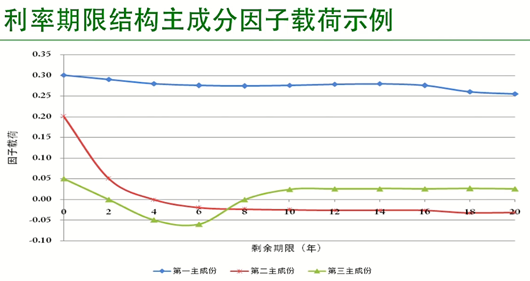
\includegraphics[width=0.8\textwidth]{fig/factor-loading.png}
	\caption{主成分因子载荷}
    \label{fig:factor-loading}
\end{figure}

\subsection{传统利率期限结构理论}

是什么原因决定了利率曲线(期限结构)的形状

\subsubsection{预期假说(Expectation Hypothesis)}

对于预期假说(Expectation Hypothesis,EH),与纯预期假说(Pure Expectation Hypothesis,PEH),或称纯预期理论(Pure Expectation Theory)或完全预期理论的区别。纯预期假设更加严格或作更强的假设,纯预期理论(PEH)认为:
\begin{itemize}
    \item 长期债券相较于短期债券的超额收益的期望为0
    \item 利率期限风险溢酬(Yield term premia)为0
    \item 远期风险溢酬(Forward term premia)为0
\end{itemize}

而预期假设(EH)对于纯预期假设有一定的放松,认为:
\begin{itemize}
    \item 长期债券相较于短期债券的超额收益的期望为常数
    \item 利率期限风险溢酬为常数
    \item 远期风险溢酬为常数
\end{itemize}

这个假说认为曲线的斜率是由于短期利率期望的改变。长期债券的较高收益反应了未来收益率上升的预期,然而长期债券的较低收益(一个向下滑动或者反向的收益率曲线)反应了短期利率下降的预期。

认为当前的利率期限结构仅代表了市场对未来即期利率变化的预期,该理论认为不存在风险溢酬,认为现实测度就是风险中性测度。看似能解释各种形状的利率期限结构,但不符合现实。投资1年期与投资30年期相比,30年之间的不确定性更大,风险更大投资者要求需要有相应的风险补偿。
由于期限结构仅包含对未来的预期,在纯预期理论认为远期利率为即期利率的现实期望,事实上两者并不相等,只有在特定测度(远期测度)下两者才会相等,而非现实测度,在现实测度下还需要加上风险溢酬。

\href{https://en.wikipedia.org/wiki/Expectations_hypothesis}{Expectation Hypothesis}

\subsubsection{流动性偏好理论(Liquidity Preference Theory)}

认为从长期利率中得到的远期利率同时反应了市场对未来的预期与流动性风险偏好,流动性偏好在这里并非指流动性风险,而是认为人们偏好短期投资,因为长期投资有利率风险(利率不确定性带来的风险)。优点是可以解释多种利率期限结构(根据不同预期),考虑了风险溢酬,但仅仅是利率风险溢酬,没有考虑其他风险的风险溢酬。

\subsubsection{市场分割理论(Market Segmentation Theory)}

投资者各有各的投资期限偏好,并且编号不变。利率曲线的形状由长、中、短期限市场各自供求关系决定。从风险溢酬的观点进行解读,可以认为投资者对投资其他期限所要求的风险溢酬无穷大,使得不改变其投资偏好,这样的设定过于极端。

\subsubsection{期限偏好理论(Preferred Habitat Theory)}

为流动性偏好理论和市场分割理论的结合,认为不同的投资者有特定期限的偏好,由于不同期限债券供求发生变化,使得风险溢酬大于所需承担的利率风险时,投资者对于期限的偏好将发生改变。从风险溢酬的观点进行解读,则该理论认为利率期限结构取决于预期和时变的风险溢酬,时变的风险溢酬又取决于期限偏好和利率风险。缺点是该理论并未解释具体的风险溢酬。

\subsection{关于期限溢酬(Term Premium)}

无风险长期利率扣除预期值之后的部分,其反映的是与利率风险相关的风险溢酬,其与利率风险的市场价格有关。理解期限溢酬可以帮助理解利率期限结构的形成和变化规律。纯预期理论的三个版本,对应着三种计算期限溢酬的方法。

\subsubsection{关于格林斯潘之谜}

1999年,联邦利率的增加伴随着长期利率一对一上升。(短端和长端一同上升)
2004年6月至2006年6月,美联储将联邦利率从1.25\%提升至5.25\%。但美国10年期国债的收益率在此期间确实下降的。(短端上升,但长端在下降)
Bernanke(2013),引用了Kim和Wright(2005)年的研究(提出了三因子无套利仿射模型,研究期限结构中长短端变化不一致的原因,发现原因为期限溢酬的影响),认为美国十年期国债收益率下降的主要原因为2010以来期限溢酬的急剧下降。

\subsubsection{纯预期理论的3个版本}

版本1:远期利率是市场对未来即期利率的预期
\begin{equation*}
	R(t,t_i,t_j) = \E_t(R(t_i,t_j))
\end{equation*}

版本2:短期零息票债券滚动投资n年的预期收益率应该等于n年期零息票债券一次性投资的收益率
\begin{equation*}
	\frac{1}{\E_t\left[e^{R(t+1,t_n)(n-1)}\right]} = e^{R(t,t+1)-R(t,t+n)\times n}
\end{equation*}

版本3:1年期零息票债券与n年期零息票债券投资1年的预期收益率应该是相等的(Local Expectation Hypothesis)
\begin{equation*}
	\E_t \left[\frac{1}{e^{R(t+1,t_n)(n-1)}}\right] = e^{R(t,t+1)-R(t,t+n)\times n}
\end{equation*}

\subsubsection{纯预期理论的错误之处}

核心问题在于其忽略了利率中的风险溢酬

版本1:根据陈蓉和郑振龙(2007),远期利率并不等于未来即期利率的期望值,两者之间还相差利率风险溢酬

版本2和版本3:虽然考虑了利率的风险,但没有考虑人们的风险厌恶系数

版本3:根据Jensen不等式,版本2与版本3之间并不等价
\begin{equation*}
	\frac{1}{\E_t\left[e^{R(t+1,t_n)(n-1)}\right]}
	\neq \E_t \left[\frac{1}{e^{R(t+1,t_n)(n-1)}}\right]
\end{equation*}

\subsubsection{Term Premium的估计}

基于远期利率的期限溢酬
\begin{equation*}
	\text{TP}_t^{1,n} = R(t,t+1,t+n) - \E_t[R(t+1,t+n)]
\end{equation*}

基于即期利率的的期限溢酬(版本2的近似)
\begin{equation*}
	\text{TP}_t^{1,n} = R(t,t+n) - \frac{1}{n} \sum^{n-1}_{i=0} \E_t[R(t+i,t+i+1)]
\end{equation*}

基于持有期收益率的期限溢酬(超额收益v,版本3近似)
\begin{align*}
	\text{TP}_t^{1,n} &= n R(t,t+n) - (n-1)\E_t[R(t+1,t+n)] - R(t,t+1) \\
	&= \E_t \left[\ln \frac{B(t+1,t+n)}{B(t,t+n)} \right] - R(t,t+1)
\end{align*}

\subsection{利率期限结构的拟合}

\subsubsection{关于直接法与间接法}

拟合期限结构的方法可分为两种:直接法与间接法。直接法使用对散点插值的方法(将散点连接起来,一定过散点)。而间接法,为对散点进行拟合法(不一定过散点,但要求理论价格与市场价格相接近)。要求拟合利率期限结构具有准确性、平滑性、稳定性和灵活性。在插值法中,由于要求利率曲线过散点,对利率本身作为自变量,进行直接插值(建模)。而对于拟合法,要求是与市场价格的定价误差最小,则是对即期利率对应的零息债券价格进行建模。

\subsubsection{直接法}

\subsubsection*{自助法(Bootstrapping)}

除了市场上少部分能直接观察到的即期利率之外,还可以采用息票剥离法,利用债券市场的数据估计出一些期限的即期利率,从而得到利率期限结构上的一些离散的点(即求解DCF债券定价公式),采用插值的方法将这些点连接起来。在美国,由于金融市场发达,利率产品多,因此散点较为密集,采用线性插值(将散点两两连接)就能获得较好的效果。在中国市场中利率产品较少,如使用线性插值无法获得较为准确的平滑的利率曲线,需要采用非线性插值的方法。

\subsubsection*{多项式插值(Polynomial interpolation)}

多项式插值是利用多项式对一组给定数据进行插值的过程。即对于一组给定的数据(如来自于采样的数据),其目的就是寻找一个恰好通过这些数据点的多项式。

\textbf{分段三次多项式插值}:假设利率为期限的三次方函数,并将利率曲线分为多段,由于是三次,每段方程都有四个未知数,即每段曲线上都需要找到四个散点(如0-2年利率曲线,选取0.5、1、1.5、2年四个散点)进而可以求解方程。与线性插值相比,高次多项式插值可以获得更为光滑的曲线,但并非次数越高越好(Runge现象,高次多项式曲线波动较大,收敛性可能存在问题),一般三次可以保证函数连续和二阶可导(远期利率为即期利率的一阶导)。

\textbf{龙格现象(Runge's Phenomenon)}:高次多项式曲线波动较大,且插值的收敛性可能存在问题
\begin{figure}[H]
    \centering
    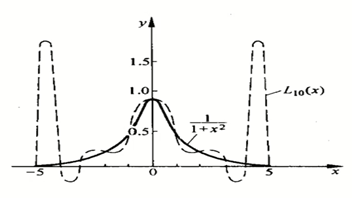
\includegraphics[width=0.8\textwidth]{fig/runges-phenomenon.png}
	\caption{龙格现象:10次Lagrange插值多项式}
    \label{fig:runges-phenomenon}
\end{figure}

\subsection*{样条插值(spline interpolation)}

样条插值为特殊的多项式插值,即使用名为样条(spline)的特殊分段多项式(piecewise polynomial)进行插值的形式。样条插值比多项式插值更加使用,用低阶的样条插值能产生高阶多项式插值类似的效果,且能避免龙格现象等数值不稳定的出现。

\begin{figure}[H]
    \centering
    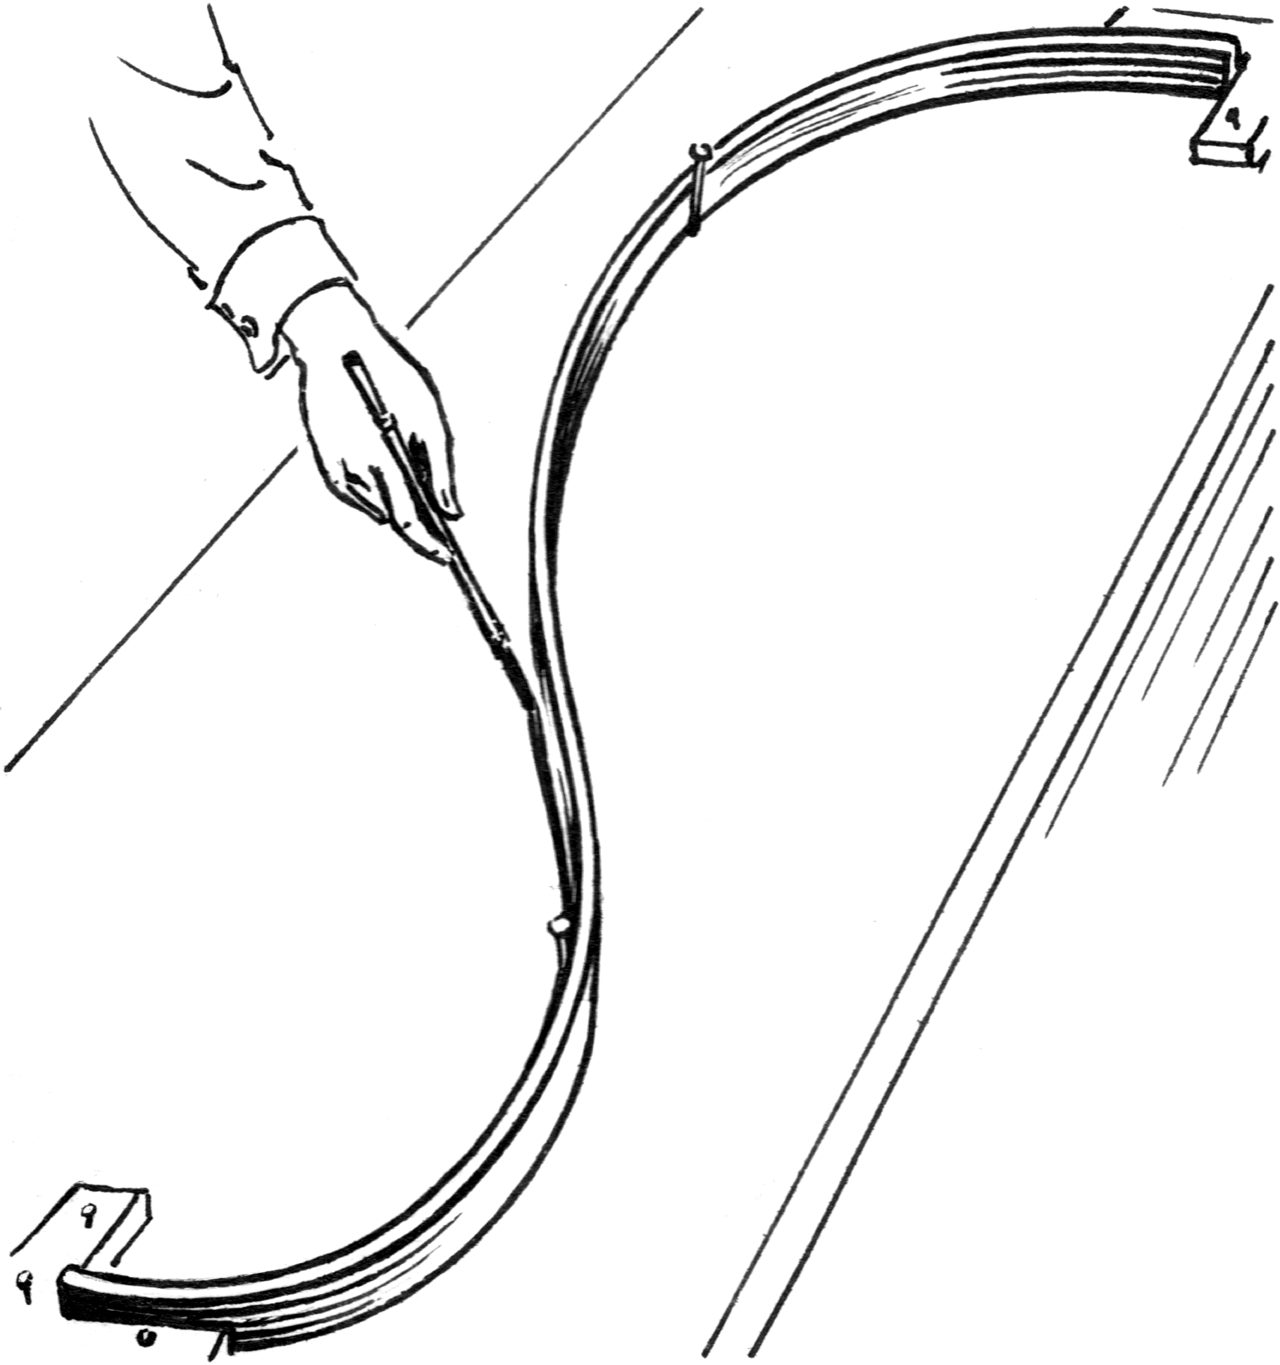
\includegraphics[width=0.8\textwidth]{fig/spline.png}
	\caption{木质样条}
    \label{fig:spline}
\end{figure}

\textbf{三次Hermite样条插值(Cubic Hermite spline)}:使用样条函数,保证分段内光滑、各段连接处也光滑。将完整区间分为n个细分区间,在每个细分区间,使用两个端点的函数值与导数值分别构建三次Hermite插值多项式,在不仅保证的节点值相等(过散点),更要求中间节点的导数(中债登要求一阶导数相等)值相等,使得一阶导连续。在任意细分区间内($p$为函数值,$m$为一阶导数值),其中有:
\begin{equation*}
	p(x) = h_{00}(t) p_k + h_{10}(t)(x_{k+1} - x_k)m_k + h_{01}(t)p_{k+1} + h_{11}(t)(x_{k+1}-x_k) m_{k+1}
\end{equation*}

\begin{equation*}
	\text{其中有}
	t=\frac{x-x_k}{x_{k+1}-x_k} \text{,且有4种Hermite basis functions为}
	\begin{cases}
		h_{00} = 2t^3 - 3t^2 +1 \\
		h_{10} = t^3 - 2t^2 + t \\
		h_{01} = -2t^3 + 3t^2\\
		h_{11} = t^3 -t^2
	\end{cases}
\end{equation*}

n段区间,n+1个节点,对应2n+2个条件(方程),可以解得2n+2个参数,对应2n+1次多项式(如3次多项式对应4个参数)。即对于1段区间,此时n=1,对应4个条件(端点函数值相等,端点一阶导数值相等),即每2个节点做一次3次Hermite插值。

\begin{figure}[H]
    \centering
    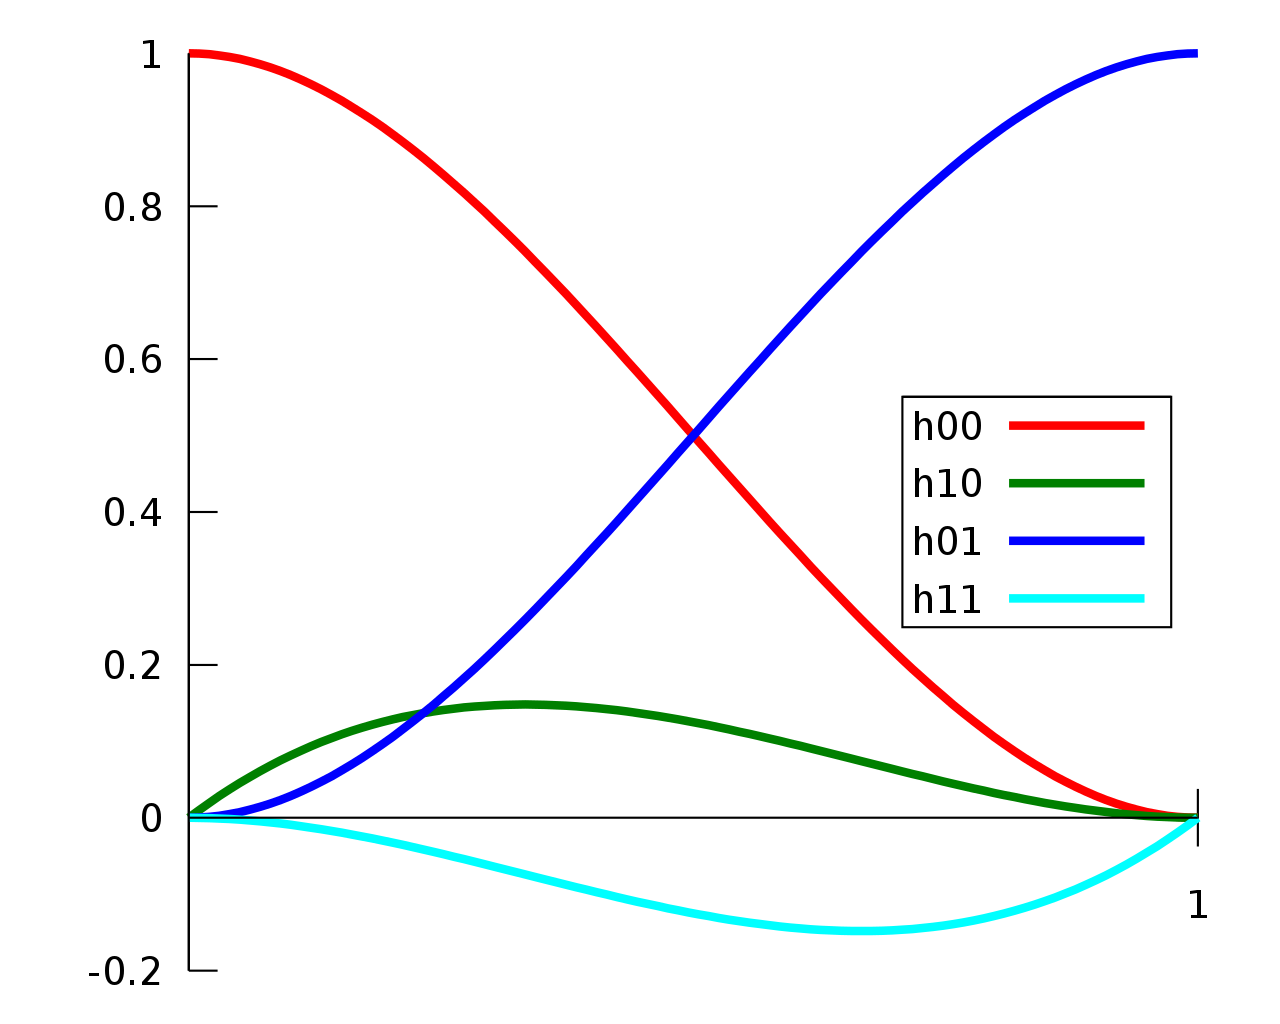
\includegraphics[width=0.8\textwidth]{fig/hermite-spline.png}
	\caption{4种Hermite基础函数}
    \label{fig:herminte-spline}
\end{figure}

\textbf{三次样条插值(Cuibc spline)}:在三次Hermite的基础上,要求在节点处二阶导数值也需相等。具体而言,将插值区间$[a,b]$分为n个区间$[(x_0,x_1),(x_1,x_2),\dots,(x_{n-1},x_n)]$。其中共有$n+1$个点,且两个端点有$x_0=a$与$x_n=b$。并在n个细分区间内,每个区间内应有三次样条函数其形式为$f_i(x) = a_i+b_i x+c_i x^2+d_i x^3\;(i=0,1,\dots,n-1)$。应满足:
\begin{enumerate}
    \item 每个细分区间$(x_i,x_{i+1})$中,$f(x)=f_i(x)$都为三次方程
    \item 满足插值条件$f(x_i) = y_i \quad (i=0,1,\dots,n)$
    \item 曲线光滑,$f(x)$、$f'(x)$与$f''(x)$连续
\end{enumerate}

此时有共有$a_i,b_i,c_i,d_i$四个未知数,并且有n个细分区间,因此要求解$4n$个未知数,需要$4n$个方程求解。除了端点$x_0=a$与$x_n=b$,其中$n-1$个中间节点都应满足前后2个细分区间内的方程$f_i(x_{i+1})=y_{i+1}$与$f_{i+1}(x_{i+1})=y_{i+1}$都通过同一中间节点,因此共有$2(n-1)$个方程。再加上两个端点属于第一个和最后一个细分区间方程$f_0(x_0)=y_0$与$f_{n-1}(x_n)=y_n$,共有$2n$个方程。

其次$n-1$个中间节点的一阶导数应该是连续的,因此有$f'_i(x_{i+1}) = f'_{i+1}(x_{i+1})$,因此共有$n-1$个方程。同理其二阶导数也应该是连续的,$f''_i(x_{i+1}) = f''_{i+1}(x_{i+1})$,因此又有$n-1$个方程。此时中间点、一阶导、二阶导等条件共有$4n-2$个方程,还需要额外的两个方程便可求解,可以通过边界条件得到,一共有3种边界条件:
\begin{enumerate}
    \item 自然边界(Natural spline):将两个端点的二阶导数设定为0,即$f''_0(x_0)=f''_{n-1}(x_n)=0$
    \item 固定边界(Clamped spline):指定端点一阶函数,设为P、Q,则有:$S'_0(x_0)=P$与$S'_{n-1}(x_n)=Q$
    \item 非扭结边界(Not-A-Knot spline):指定第一个中间节点的三阶导数与起始端点的三阶导数相同,即$f'''_1(x_1)=f'''_0(x_0)$。同时指定最后一个中间节点与终止端点的三阶导数相同,即$f'''_{n-2}(x_{n-1})=f'''_{n-1}(x_n)$。
\end{enumerate}

参考:https://zhuanlan.zhihu.com/p/62860859

\subsubsection{间接法}

\subsubsection*{贴现函数法与即期利率法对比}

贴现函数用多个连接的分段函数去逼近整条利率期限结构,精确性较高。而即期利率法经济含义明确,而且由于用一个函数拟合整条利率期限结构,曲线平滑性较好。

\subsubsection{贴现函数法(拟合法)}

并不考虑直接过散点,而是考虑如3次函数,有四个参数,对市场上的债券定价,使得其定价误差的平方和最小。贴现函数设定为样条函数(spline functions),常用的样条函数包括三次多项式样条、三次基样条(B-Spline)和三次指数样条。对于阶数的选择三次最为常见,可保证函数连续和二阶可导,对于样条数量的选择,样条数量越多拟合效果越好,但对应平滑性较差,也容易受到异常点的影响。对于节点的选择一般需使得每段区间具有一定的经济意义,样本数量较为接近。在参数校准的过程中,需要先写出债券价格P与不同期限零息债价格的函数(定价公式),而零星债券价格又可以如上写成与期限s的函数,因此最终可写成$P$与$s$的函数,同时需要估计参数$\beta$,使得定价误差的平方和$\varepsilon_1^2+\varepsilon_2^2+\varepsilon_3^2+⋯$最小,即线性最小二乘法,($V(\beta)$为债券的理论价值,为$s$的函数)。但此时存在异方差问题,即期限短的债券,定价误差小,而期限长的债券,定价误差大。一般解决方法为直接设定方差与期限平方或久期平方成比例。在加入约束条件的情况下,需要使用GLS而非OLS。

\subsubsection*{贴现函数法:参数校准}

参数校准:
\begin{equation*}
	\bm{\hat{\beta}} = \argmin_{\hat{\beta}} \sum^n_{j=1}\left(P^j - V^j\right)^2
\end{equation*}

在线性回归中,回归系数的最小二乘估计就是使得回归方程残差平方和最小的系数值。因此,只要对贴现函数形式的设定使得理论价值能表达为参数的线性形式,参数的校准过程就等价于对回归方程的线性回归过程:
\begin{equation*}
	\mathbf{P=V(\bm{\beta})+\bm{\varepsilon}}
\end{equation*}

\begin{equation*}
    \E(\varepsilon)=0,\,\Cov(\varepsilon_{t_i},\varepsilon_{t_j}),\,\Var(\varepsilon) = \Sigma^2\Omega = \sigma^2
    \begin{bmatrix}
        w_1^2 & 0 & \cdots & 0 \\
        0 & w_2^2 & \cdots & 0 \\
        \vdots & \vdots & \ddots & \vdots \\
        0 & 0 & \cdots & w_n^2
    \end{bmatrix}
\end{equation*}

\subsubsection{即期利率函数法(拟合法)}

认为插值法和拟合法都是单纯使用数学公式,缺陷在为内在经济含义不足。由于已经不是线性函数,因此在对模型参数时,只能使用非线性最优化技术,并且同样需要考虑异方差和约束条件。

\subsubsection*{Nelson-Siegel(NS)模型}

函数自变量为s,其中有待估参数$\beta_0,\beta_1,\beta_2,m$。三个参数分别对应着利率期限结构中的水平变化、斜率变化以及曲度变化,可以看到其待估参数与主成分分析之间纯在这自然的联系,短期利率由$\beta_0,\beta_1$决定,而长期利率只由$\beta_0$决定,因此在NS模型下,短期利率的波动率比长期利率的波动率大,与实际相符,其缺陷在于NS可以拟合的曲线形状有限。

指数形式的瞬时远期利率:
\begin{equation*}
    f(0,s)=\beta_0+\beta_1 e^{-\frac{s}{m}}+\beta_2\frac{m}{s}e^{-\frac{s}{m}}
\end{equation*}

对应的即期利率函数:
\begin{align*}
    R(0,s) &= \frac{1}{s}\int^s_0 f(0,\tau)d\tau \\
    &= \beta_0 + \beta_1 \frac{1-e^{-\frac{s}{m}}}{s/m} + \beta_2\left[\frac{1-e^{-\frac{s}{m}}}{s/m} - e^{-\frac{s}{m}}\right]
\end{align*}

NS参数的经济含义:
\begin{itemize}
    \item $\beta_0$:长期因子:期限无穷大时利率收敛于$\beta_0$。水平因子:载荷为1,1是不衰减的常数,对所有期限利率影响一致
    \item $\beta_1$:短期因子:其载荷是一个开始于1,并很快衰减至0的函数,对短期利率影响大。斜率因子:当期限趋于0时,$\beta_1=R(0,0)-\beta_0$,因此也可以看作是长短期利率之差(spread)
    \item $\beta_2$:其载荷开始于0先增加后衰减为0,对中期利率影响大,主要影响收益率曲线的弯曲度,通常被称为“中期因子”或“曲度因子
    \item $m$:决定了$\beta_1$和$\beta_2$,的衰减速度。如果$m$较小,收敛的速率比较快,能较好地拟合较长到期期限的曲线。$m$较大时,收敛的速度较慢,能比较好地拟合较短到期期限的收益率曲线
\end{itemize}

\subsubsection*{Nelson-Siegel-Svensson(NSS)模型}

改进NS模型中刻画曲线种类受限的问题,在NS模型的基础上增加了中期项,并增加待估曲度参数$\beta_3$和调整参数$m_2$,使得中短部分的形状更为灵活多样,能够刻画出更丰富形状的利率期限结构。

即期利率函数
\begin{equation*}
    R(0,s) = \beta_0 + \beta_1 \frac{1-e^{-\frac{s}{m_1}}}{s/m_1} + 
    \beta_2\left[\frac{1-e^{-\frac{s}{m_1}}}{s/m_1} - e^{-\frac{s}{m_1}}\right] +
    \beta_3\left[\frac{1-e^{-\frac{s}{m_2}}}{s/m_2} - e^{-\frac{s}{m_2}} \right]
\end{equation*}

\subsubsection*{即期利率函数法:参数校准}

\begin{itemize}
    \item 无法使用最小二乘法,而只能使用非线性最优化技术
    \item 同样需要考虑异方差和约束问题
    \item 异方差调整通过赋予短期债券较大的权重来体现
\end{itemize}

\begin{align*}
    \bm{\hat{\beta}} &= \argmin_{\hat{\beta}} \sum^n_{j=1}\left(\frac{P^j - V^j}{w_j}\right)^2 \\
    w_j &= \frac{dP_j}{dy_j}
\end{align*}

\end{document}